\section{Исследовательская часть}

\subsection{Эволюционный алгоритм}

Теоретическое обоснование генетических алгоритмов приводится в работе Дж. Холланда [1]. 
Ключевой является теорема схем, доказывающая эффективность генетического алгоритма. Теорема схем показывает происходящее при смене поколений экспоненциальное распространение хорошо приспособленных схем.

Эта теорема, вкупе с решением задачи многорукого бандита [3] показывает, что генетические алгоритмы являются наиболее быстрым методом поиска в пространствах с неизвестными свойствами.

Теорема схем формулируется для представления генома в виде битовых строк фиксированной длины.

Для обоснованности применения данной теоремы к деревьям вычисления достаточно ввести ограничение на максимальную глубину дерева, добавить некоторый виртуальный оператор-заглушку и добавив виртуальные параметры привести все операторы к одной арности. В таком случае все деревья будут иметь одинаковую структуру и количество узлов. Тогда их можно взаимно отобразить в бинарные строки фиксированной длины и структуры. Таким образом, теорема схем применима и в случае деревьев вычислений.

\clearpage
\subsubsection{Алгоритм скрещивания} \label{sssec:crossover}
В разрабатываемом модуле эволюционирующей структурой является дерево вычислений. Это влечёт за собой отличия от классического генетического алгоритма, применяемого к битовым строкам или массивам.

Хотя формулу можно представить в виде строки, скрещивание напрямую двух строк одноточечным или многоточеченым скрещиванием является крайне неэффективным методом, так как при этом нарушается вложенность скобок, разрываются операция и её аргументы и подавляющее большинство формул-потомков являются некорректными и невычислимыми.

\begin{figure}[!h]
\centering
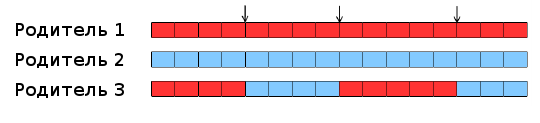
\includegraphics[scale=0.7]{research/pics/1.png}
\caption{Иллюстрация многоточечного скрещивания массива..}
\label{figure:arrayCrossover}
\end{figure}


По этой причине была выбрана схема скрещивания поддеревьями. Формула представляется в виде дерева вычислений. Для скрещивания в каждом дереве выбирается узел. Каждый выбранный узел – корень некоторого поддерева. Скрещивающиеся деревья обмениваются соответствующими поддеревьями, образуя пару потомков.

Пример: скрещивание деревьев, описывающих формулы 

  sin(X0^2)+X1*2.3

  sqrt(X0/3.14)*(X1+X0^2)

с корнями поддеревьев в +, \^{} (возведение в степень) соответственно, даёт:

  sin(X0 + 1) + X1 * 2.3

  sqrt(X0 / 3.14) * (X1 + X0 + 1)

\clearpage
\begin{figure}[!h]
\centering
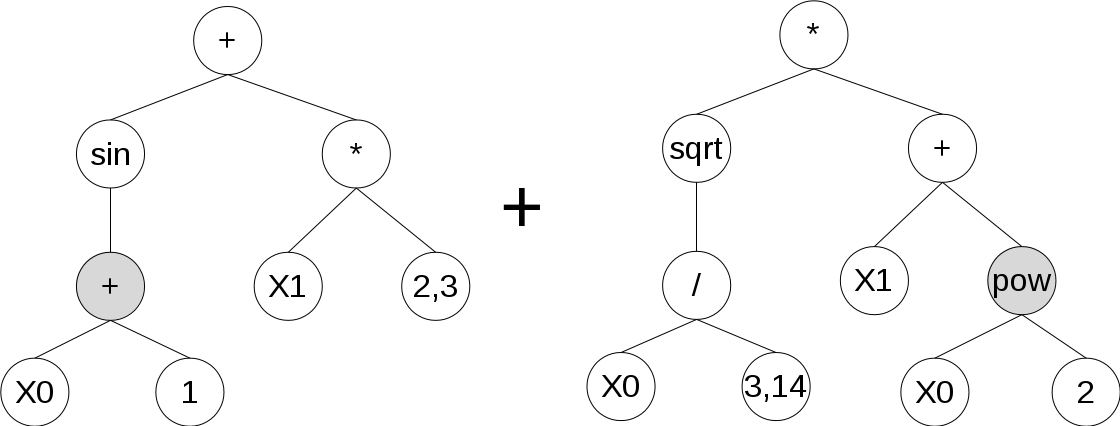
\includegraphics[scale=0.5]{research/pics/2.png}

=

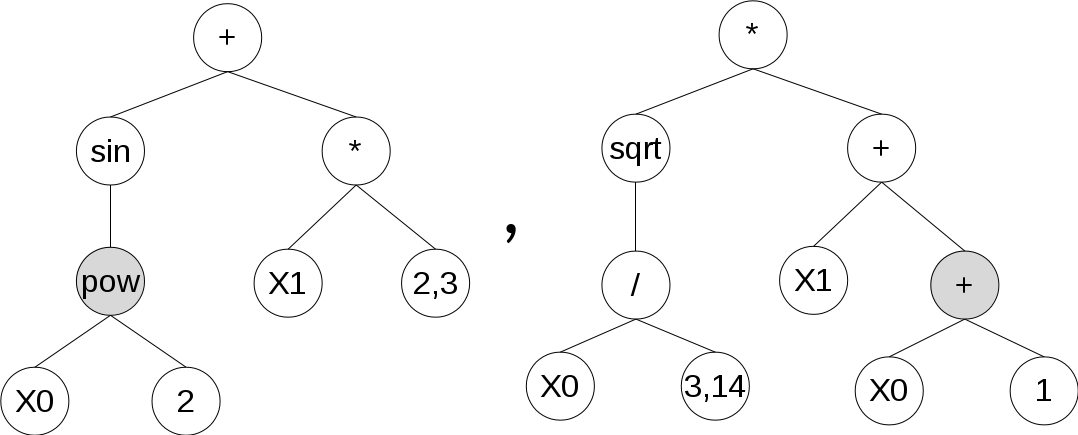
\includegraphics[scale=0.5]{research/pics/3.png}
\label{figure:crossover}
\caption{Пример скрещивания деревьев}
\end{figure}

У такого метода скрещивания есть одна особенность. Если у первого родителя можно выбирать абсолютно любой узел, то для второго родителя такой подход может вести к превышению максимально допустимой глубины. Проиллюстрируем примером:

Возьмём деревья из предыдущего примера и установим максимально допустимую глубину дерева = 4. Оба родителя выполняют это условие. 

Будем выбирать случайные узлы у обоих родителей. Может сложиться такая ситуация:

\clearpage
\begin{figure}[!h]
\centering
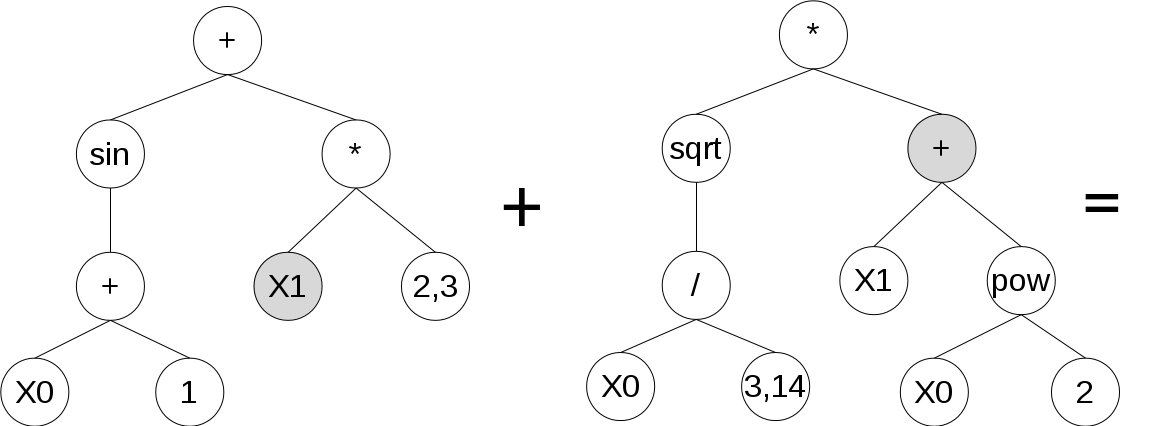
\includegraphics[scale=0.5]{research/pics/4.png}

=

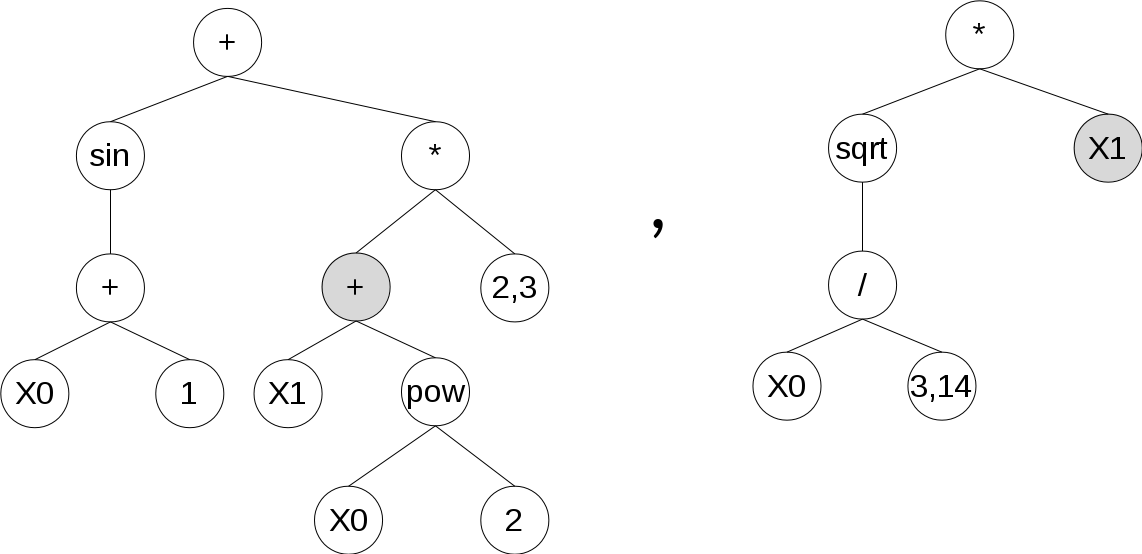
\includegraphics[scale=0.5]{research/pics/5.png}
\label{figure:crossoverOverflow}
\end{figure}

Как мы видим, несмотря на то что после скрещивания получились корректные с математической точки зрения формулы, первое дерево превысило максимально допустимую глубину.

Происходит это из за серьёзного отличия от скрещивания массивов. В случае массивов  оба родителя имеют одинаковую структуру и длину. Поэтому точка, выбранная на одном массиве, имеется и на другом, и, обменяв эти точки, мы получаем заведомо подоходящих по структуре и длине потомков. 

Деревья-родители же имеют различную структуру и размеры. Поэтому такой подход в принципе не возможен. 

Чтобы избежать разрастания в глубину, для второго дерева выбор узлов для обмена должен осуществляться только среди таких узлов, при выборе которых не нарушится ограничение по глубине -- <<хороших>> узлов.

\subsubsection{Поиск «хороших» узлов}

Для рассуждений в данном случае деревья удобнее представлять как линейные структуры. Общее правило от этого не изменится.

Точки 2 и 4 обозначают глубину первого и второго дерева соответственно.

Точки 1 и 3 обозначают выбранные для скрещивания 

d1, d2 -- глубина точек 1 и 3.

h1, h2 -- высота точек 1 и 3.

\begin{figure}[!h]
\centering
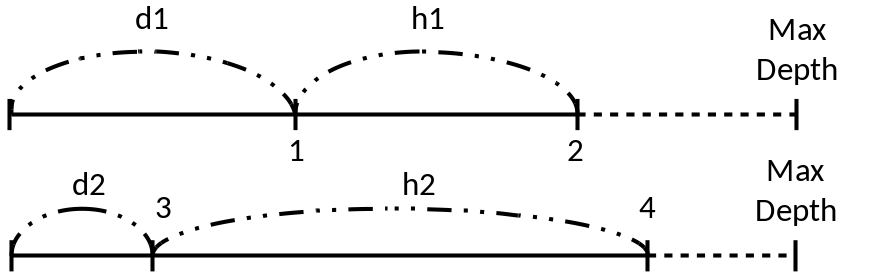
\includegraphics[scale=0.7]{research/pics/6.png}
\label{figure:arrayGoodNodes1}
\end{figure}

Условие, что глубины деревьев-родителей меньше максимальной:

\begin{equation}
\label{equation:goodNodesEq1}
\begin{cases} d1 + h1 \leq Max_{depth} \\ d2 + h2 \leq Max_{depth} \end{cases}
\end{equation}

После скрещивания получим новые деревья. 

\begin{figure}[!h]
\centering
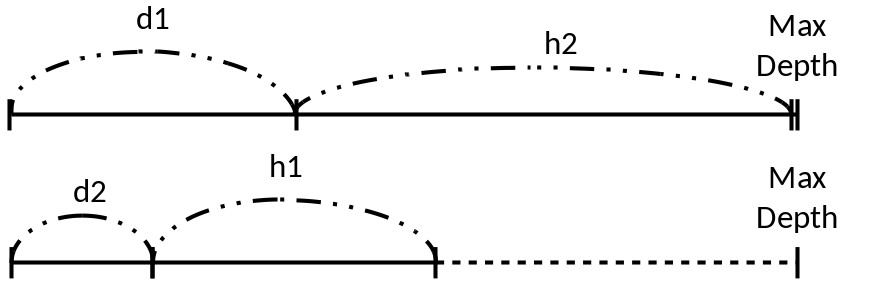
\includegraphics[scale=0.7]{research/pics/7.png}
\label{figure:arrayGoodNodes2}
\end{figure}

Запишем условие по глубине:

\begin{equation}
\label{equation:goodNodesEq2}
\begin{cases}d2 + h1 \leq Max_{depth} \\  d1 + h2 \leq Max_{depth} \end{cases}
\end{equation}

\clearpage
Отсюда получим условие для подходящих узлов:

\begin{equation}
\label{equation:goodNodesEq3}
\begin{cases} d2 \leq Max_{depth} - h1 \\ h2 \leq Max_{depth} - d1  \end{cases}
\end{equation}

Все узлы, удовлетворяющие условию \ref{equation:goodNodesEq3}, являются «хорошими». Выбор узла среди них осуществляется случайным образом.

\subsubsection{Алгоритм мутации}

Мутация -- одна из ключевых операций эволюционного алгоритма.

В подсистеме применяется следующий алгоритм мутации:
\begin{enumerate}
\item Случайным образом выбирается узел дерева. Вероятность выбора для всех узлов дерева одинакова.
\item Выбранный узел, вместе с его поддеревом, заменяется на новое поддерево, генерируемое по общим правилам, с учётом условия на максимальную глубину. 
\end{enumerate}

\clearpage
\begin{figure}[!h]
\centering
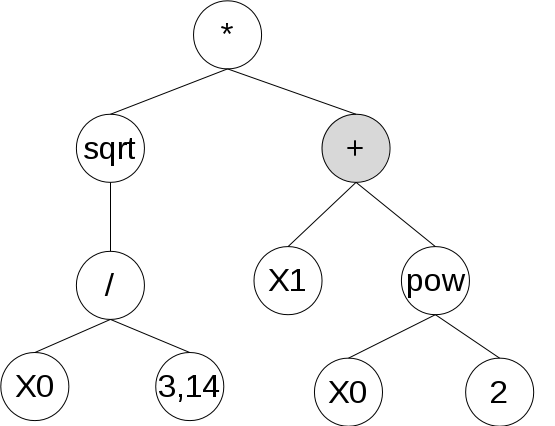
\includegraphics[scale=0.7]{research/pics/8.png}

=>

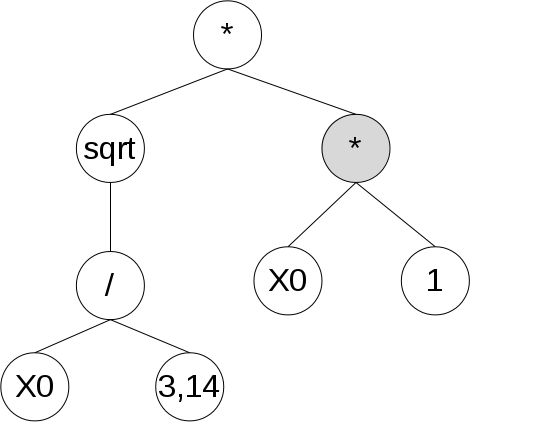
\includegraphics[scale=0.7]{research/pics/9.png}
\label{figure:mutation}
\caption{Пример мутации}
\end{figure}

Для осуществления этого, необходимо реализовать равномерное распределение вероятностей для узлов графа. Что является интересной задачей, учитывая, что алгоритм выбора узлов должен быть рекурсивным и что дерево – структура данных без случайного доступа. 


\clearpage
\subsubsection{Равномерное распределение на узлах дерева}

Выбор с одинаковой вероятностью среди узлов дерева реализовывается таким образом:

В каждом узле хранится числова характеристика offs, которая равна количеству всех потомков узла + 1 (сам узел). Количество потомков расчитывается рекурсивно:

\begin{equation}
\label{equation:goodNodesEq3}
offs(ind) = \begin{cases} 1, & \mbox{для листьев дерева} \\ 1 + \sum_i(offs(child_i)), & \mbox{для прочих вершин} \end{cases}
\end{equation}

Выбор осуществляется с корневого узла дерева. Алгоритм выбора приведён далее.

\clearpage
\begin{figure}[!h]
\centering
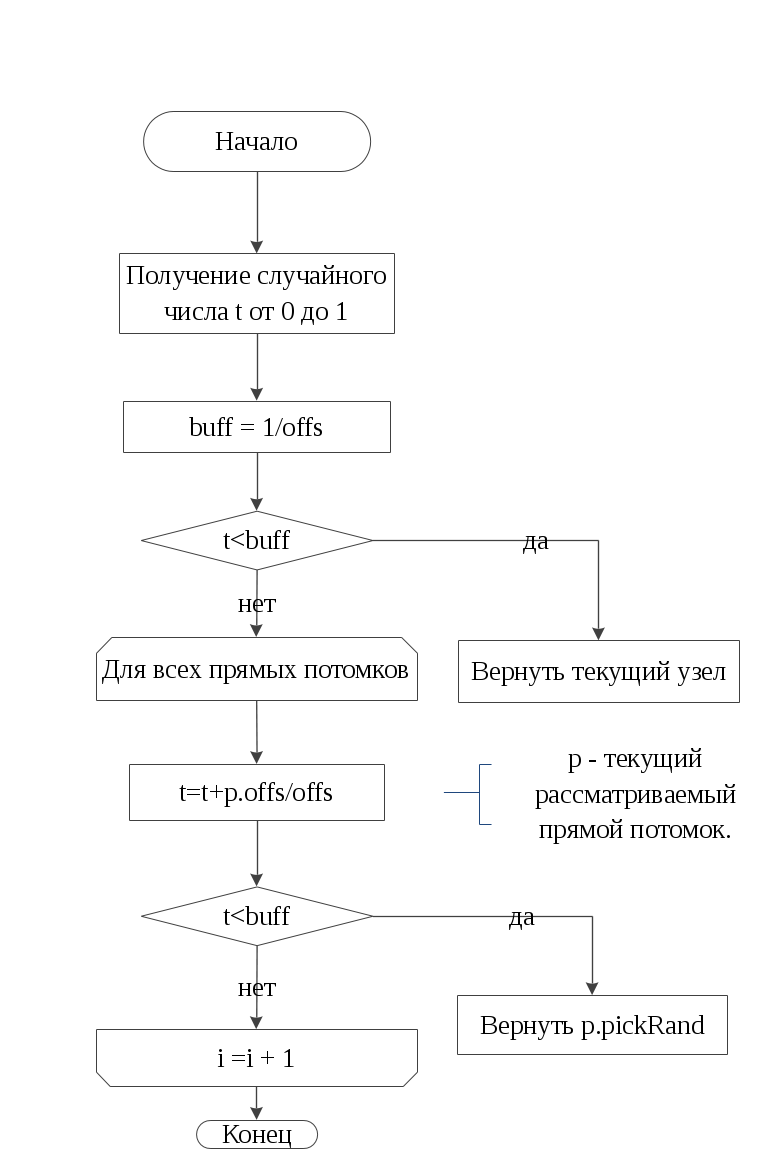
\includegraphics[scale=0.7]{research/pics/12.png}
\label{figure:randomPick}
\end{figure}

\clearpage
Проверим алгоритм:


\begin{figure}[!h]
\centering
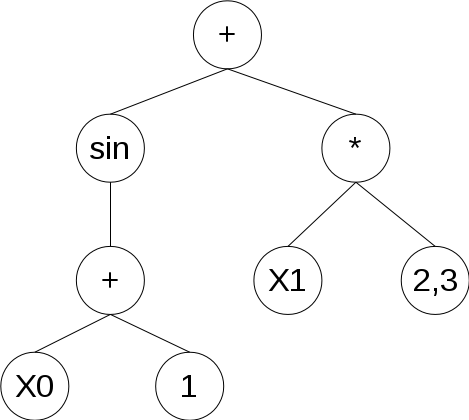
\includegraphics[scale=0.4]{research/pics/10.png}
\caption{Дерево}
\label{figure:offsTree1}
\end{figure}
\begin{figure}[!h]
\centering
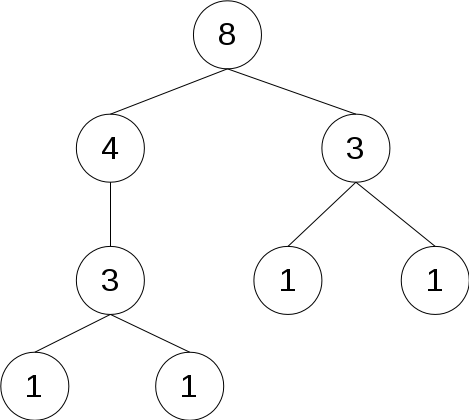
\includegraphics[scale=0.4]{research/pics/11.png}
\caption{Дерево offs}
\label{figure:offsTree2}
\end{figure}

Для дерева \ref{figure:offsTree1} вероятность выбрать любой узел должна равняться $\frac{1}{8}$.

\renewcommand{\arraystretch}{1.5}

\begin{table}[h!]
\centering
\caption{Вероятность выбора узла}
\begin{tabular}{L{4cm}|L{8cm}}
\multicolumn{1}{C{4cm}|}{Узел} & 
\multicolumn{1}{C{8cm}}{Вероятность} \\
\hline\hline

Корень & $\frac{1}{8}$ \\ \hline
sin & $\frac{4}{8} \cdot \frac{1}{4} = \frac{1}{8}$ \\ \hline
+ & $\frac{4}{8} \cdot \frac{3}{4} \cdot \frac{1}{3} = \frac{1}{8}$ \\ \hline
X0 & $\frac{4}{8} \cdot \frac{3}{4} \cdot \frac{2}{3} \cdot \frac{1}{2} = \frac{1}{8}$ \\ \hline
1 & $\frac{4}{8} \cdot \frac{3}{4} \cdot \frac{2}{3} \cdot \frac{1}{2} = \frac{1}{8}$ \\ \hline
* & $\frac{3}{8} \cdot \frac{1}{3} = \frac{1}{8}$ \\ \hline
X1 & $\frac{3}{8} \cdot \frac{2}{3} \cdot \frac{1}{2} = \frac{1}{8}$ \\ \hline
2.3 & $\frac{3}{8} \cdot \frac{2}{3} \cdot \frac{1}{2} = \frac{1}{8}$ \\ \hline

\end{tabular}
\end{table}

Как видим, для всех узлов вероятность выбора = $\frac{1}{8}$.

Так же вполне очевидно, что это правило работает и в общем случае.

\subsubsection{Выбор стратегии скрещивания}

Скрещивание двух деревьев описано в пункте \ref{sssec:crossover}. Встаёт вопрос выбора конкретных родителей из множества всех индивидов.

Возможны различные способы выбора, основанные на идее, что индивид с большим значением приспособленности, должен иметь больший шанс дать потомство.

Некоторые из способов:
\begin{itemize}
\item Пропорциональный
\item Состязание
\end{itemize}

Опишем каждый из них в отдельности.

\paragraph{Пропорциональный} \label{par:prop}

Для каждого индивида рассчитывается вероятность оставить потомство.

\begin{equation}
\label{equation:propF1}
p_i = \frac{f_i}{\sum_{j=1}^N(f_j)}
\end{equation}
\begin{ESKDexplanation}
\item[где ] $f_i$ -- приспособленность i-го индивида,
\item $N$ -- количество индивидов
\end{ESKDexplanation}

Выполняется условие:

\begin{equation}
\label{equation:propF1}
\sum_{i=1}^N(p_i) = 1
\end{equation}

Выбираются 2 родителя согласно описанному распределению вероятностей и дают 2 потомка, которые добавляются в новое поколение. 

Эти действия повторяются, пока новое поколение не будет заполнено.

\paragraph{Состязание}

Моделируется такое явление живой природы, как бои за право спаривания.

Выбираются два случайных индивида, и проводится «состязание». Индивид с наибольшим значением фитнеса считается победителем.

Выбирается вторая пара и определяется второй победитель.

Победители образуют пару и дают потомство.

\paragraph{Выбор стратегии}

Критерии:

\begin{itemize}
\item Вычислительная сложность
\item Затраты памяти
\item Скорость схождения
\end{itemize}

Сравнение проведём по методу Борда

\begin{table}[h!]
\centering
\caption{Сравнение стратегий}
\begin{tabular}{L{5cm}|L{5cm}|L{5cm}}
\multicolumn{1}{C{5cm}|}{Критерий} & 
\multicolumn{1}{C{5cm}|}{Пропорциональный} &
\multicolumn{1}{C{5cm}}{Состязание} \\
\hline\hline

Вычислительная сложность & 2 & 1 \\ \hline
Затраты памяти & 1.5 & 1.5 \\ \hline
Скорость схождения & 1.5 & 3 \\ \hline
Итоговый ранг & 5 & 5.5 \\
\end{tabular}
\end{table}

Согласно сравнению следует предпочесть пропорциональную стратегию.

\subsubsection{Выбор критериев качества}
Критерием качества для найденного решения будет служить среднеквадратичная ошибка:

\begin{equation}
\label{equation:geneticsMSE}
MSE = \frac{1}{N}\sqrt{\sum_{i=1}^N(ind_f(x_1^i ... x_m^i) - y^i)^2}
\end{equation}
\begin{ESKDexplanation}
\item[где ] $ind_f(x_1^i ... x_m^i)$ -- значение функции индивида в точке $(x_1^i ... x_m^i)$,
\item $y$ -- значение из обучающей выборке в точке $i$
\item $N$ -- количество точек в обучающей выборке
\item $m$ -- размерность пространства поиска
\end{ESKDexplanation}

Функция приспособленности в таком случае будет рассчитываться как

\begin{equation}
\label{equation:geneticsFit}
f = \frac{1}{MSE}
\end{equation}